
\documentclass{standalone}
\usepackage{tikz}
\usetikzlibrary{arrows.meta,calc,decorations.pathmorphing}
\usepackage{xcolor}
\definecolor{colorff6633}{HTML}{ff6633}
\begin{document}
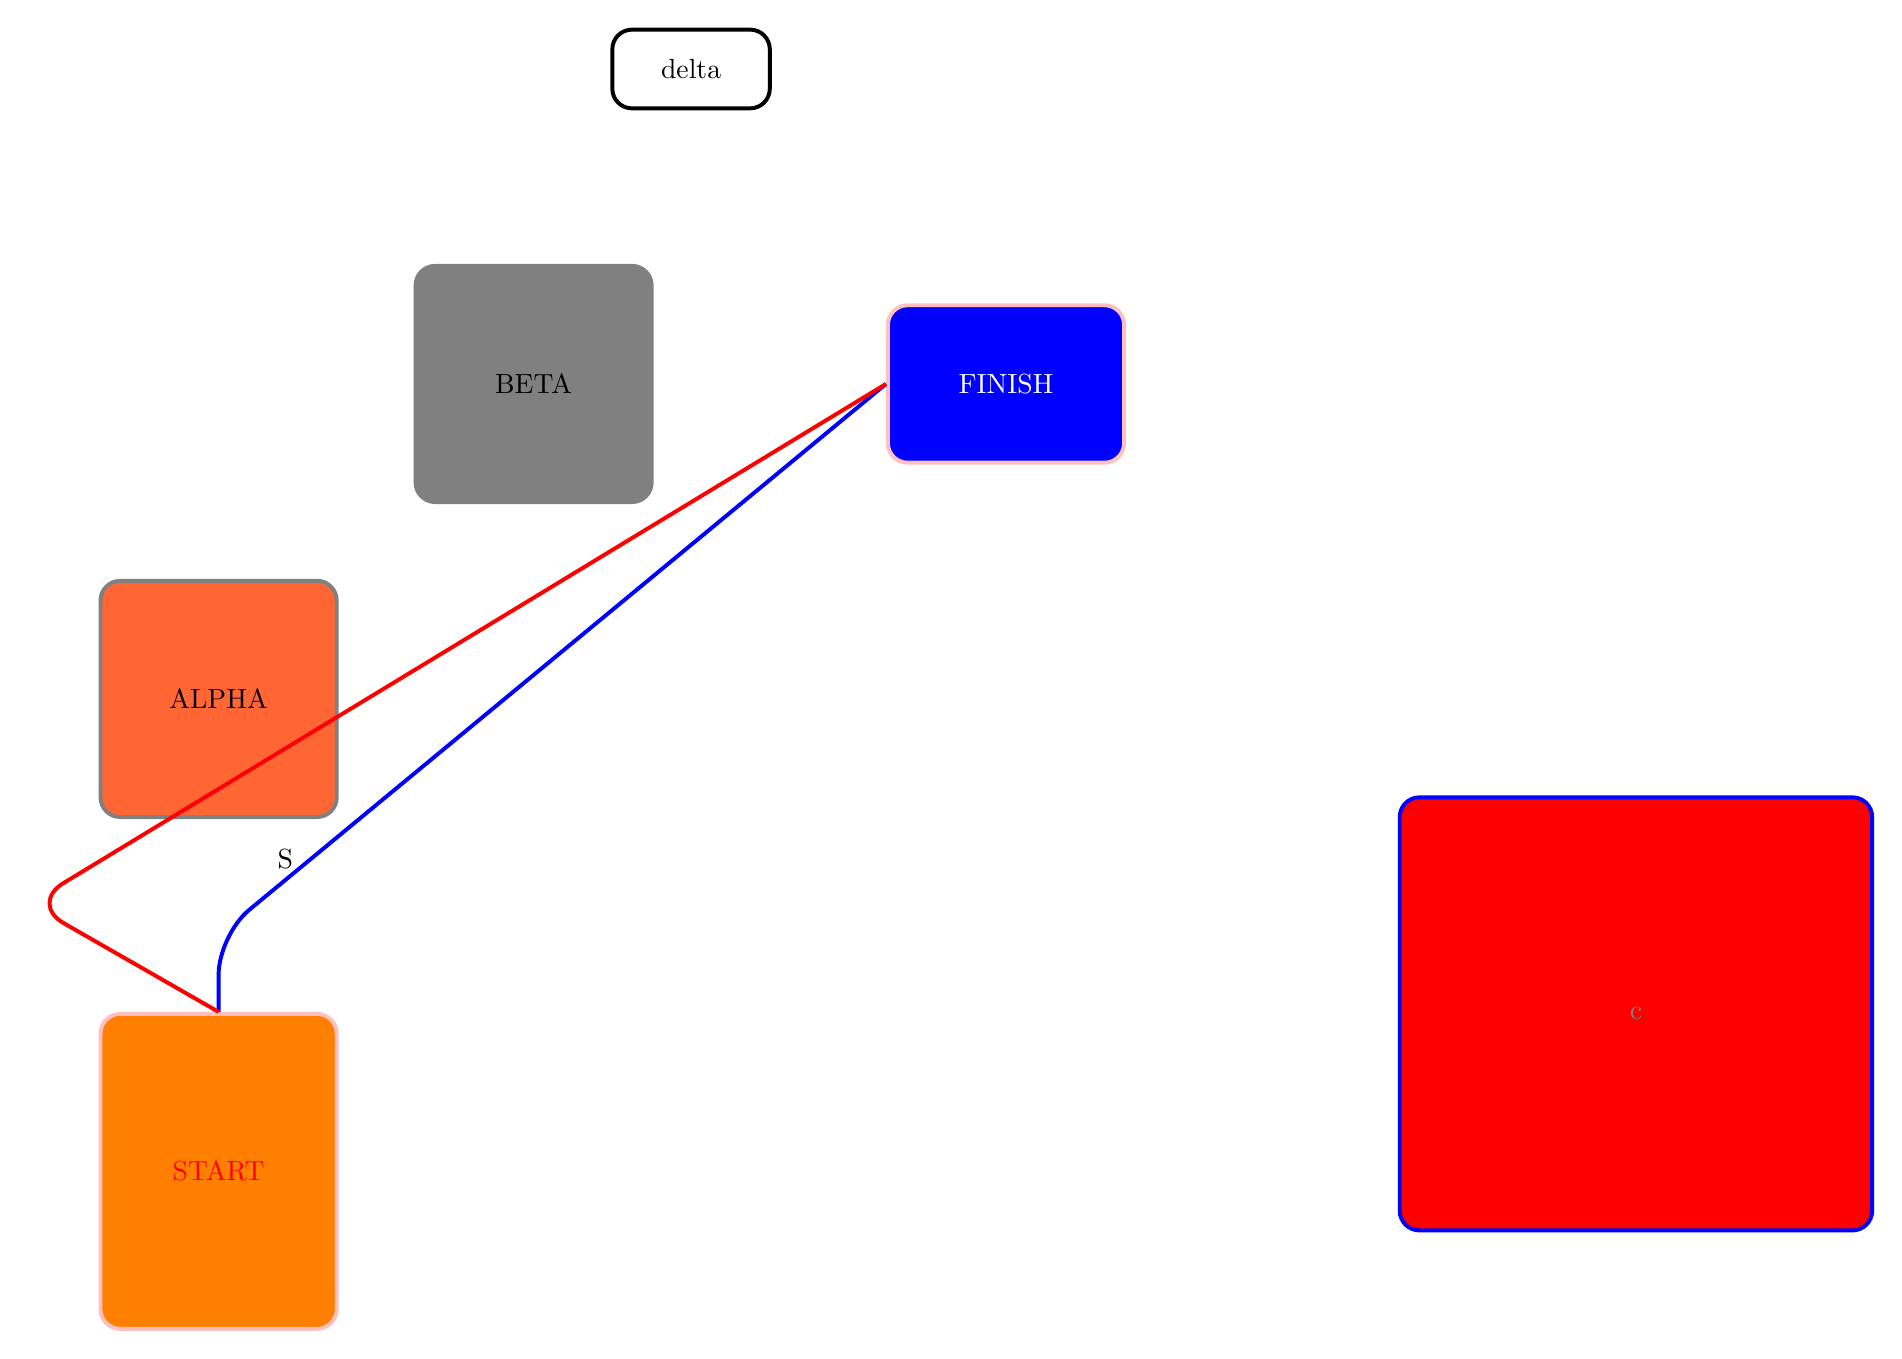
\begin{tikzpicture}
    [>={Stealth[scale=1.0]},  % Uniform arrow style
    ]
    
\node[rectangle, fill=orange, draw=pink, minimum width=3cm, minimum height=4cm, rounded corners=0.25cm, line width=0.05cm] (node_a) at (4,4) {\textcolor{red}{START}};
\node[rectangle, fill=blue, draw=pink, minimum width=3cm, minimum height=2cm, rounded corners=0.25cm, line width=0.05cm] (node_b) at (14,14) {\textcolor{white}{FINISH}};
\node[rectangle, fill=red, draw=blue, minimum width=6cm, minimum height=5.5cm, rounded corners=0.25cm, line width=0.05cm] (node_c) at (22,6) {\textcolor{gray}{c}};
\node[rectangle, fill=colorff6633, draw=gray, minimum width=3cm, minimum height=3cm, rounded corners=0.25cm, line width=0.05cm] (node_alpha) at (4,10) {ALPHA};
\node[rectangle, fill=gray, draw=gray, minimum width=3cm, minimum height=3cm, rounded corners=0.25cm, line width=0.05cm] (node_beta) at (8,14) {BETA};
\node[rectangle, fill=white, draw=black, minimum width=2cm, minimum height=1cm, rounded corners=0.25cm, line width=0.05cm] (node_delta) at (10,18) {delta};
\draw[draw=blue,line width=0.05cm,rounded corners=0.5cm] (node_a.north) -- (4,7) -- (node_b.west) node[above, pos=0.1] {S};
\draw[draw=red,line width=0.05cm,rounded corners=0.5cm] (node_a.north) -- (1.6,7.4) -- (node_b.west);

\end{tikzpicture}
\end{document}
